%% stevensThesis.tex
%% Copyright 2008 B. E. Arnett
%
% ----->  Latex is not required for writing your dissertation or thesis.  Most theses are done in Word or WYSIWYG editors
%------>  Latex is frequently used in math, physics and computer science for ease in producing formulas.  
%------>  This template is provided for Latex users to help in the formatting of the thesis or dissertation.  
%
%
% This work may be distributed and/or modified under the
% conditions of the LaTeX Project Public License, either version 1.3
% of this license or (at your option) any later version.
% The latest version of this license is in
%   http://www.latex-project.org/lppl.txt
% and version 1.3 or later is part of all distributions of LaTeX
% version 2005/12/01 or later.
%
% This work has the LPPL maintenance status `maintained'.
% 
% The Current Maintainer of this work is Barbara Arnett.
%
% This work consists of the files stevensthesis_num.tex 
% and the derived file pgnumchapter_nums.sty.

%
% This is the template for dissertation / thesis submission for the
% Stevens Institute of Technology.  
%
% There are fields in titlepg.sty that must be updated with your
% own information.  The file pgnumchapter.sty must be included but  
% does not need to be updated, unless you want to change the 
% layout of your pages and chapters.  
%
% Both dissertations and master thesis can created from this program.  
% These fields should be changed:
%    {thesistype} should be either "dissertation" or "thesis" 
%    {thesisdegree} should be either "doctor of philosophy" for dissertation or
%            "Master of Engineering - Electrical Engineering" 
%            "Master of Science - Computer Science"   or the correct degree designation.
%
%
% Please see the formatting instructions on the library website at
%        http://www.stevens.edu/library/services/thesis.html
%
% copyright 2007, Barbara Arnett, web services librarian, stevens institute of technology
% any comments or corrections can be sent to barnett@stevens.edu
%
% update January 2009 - updated font size to 12p and added subsections to show up in the 
% table of contents 
%
% update April 2009 - added optional dedication page, code courtesy of James Weatherall
%
% update May 2009 - added code to include the abstract, acknowledgment, dedication and vita
% 						to the table of contents.  As per Doris Oliver, everything except the title page,
% 						copyright page, and table of contents should appear in the table of contents.
%
% update July 2009 - added code to pgnumchapter_nums.sty to have top of table of contents, figures & symbols
% start 1.5 inches from the top.
%
% update February 2010 - added \bibliography and BibTex file 
%
% update May 2010 - added line to ensure Table of Contents prints in normalsize font when run in Linux
%                            also changed copyright text to say C YYYY, name. All rights reserved.
% update February 2011 - removed line \renewcommand{\thesubsection}{\thesection\arabic{subsection}}
%            to allow toc subsections to print normally (see bea02152011)

\documentclass[12pt]{report}
\usepackage {fancyhdr}
\usepackage{helvet}
\renewcommand{\familydefault}{\sfdefault}
\usepackage{graphicx, amssymb, changepage}
\usepackage{rotating}
\usepackage{setspace}
\usepackage{pgnumchapter_nums}
\usepackage{titlepg}
% algorithm2e for algorithms
\usepackage[linesnumbered,boxed, algochapter]{algorithm2e}
% For citations
\usepackage{natbib}
% To use align and gather functions
\usepackage{amsmath}
\usepackage{mathtools}
\usepackage{tocloft} % the tocloft package lets you redefine the Table of Contents (ToC)
  \renewcommand\cftchappresnum{Chapter } % prefix "Chapter " to chapter number in ToC
  \renewcommand{\cftdot}{}
  \cftsetindents{chapter}{0em}{8em}      % set amount of indenting
  \cftsetindents{section}{2em}{6em}
  \cftsetindents{subsection}{2em}{6em}
  \cftsetindents{subsubsection}{2em}{6em}

% For URL and other links
\usepackage{hyperref}
%              this is for the list of symbols page, if desired
\def\listofsymbols{%   This is the file for symbols used in the paper.
%
%\addnotation \alpha: {some variable that means something to me}{alpha}
%\addnotation \Omega: {abstract probability space}{alpha}


%%%%%%%%%%%%%%%%%%%%%%%
%Sample List of Symbols
%%%%%%%%%%%%%%%%%%%%%%%
\begin{tabbing}
% YOU NEED TO ADD THE FIRST ONE MANUALLY TO ADJUST THE TABBING AND SPACES
\hspace{5mm}$n$~~~~~\=\parbox{5in}{Vector size\dotfill \pageref{symbol:nml}}\\
%ADD THE REST OF SYMBOLS WITH THE HELP OF MACRO
\hspace{5mm}\addsymbol m: {Vector size}{symbol:nml}
\hspace{5mm}\addsymbol l: {Vector size}{symbol:nml}
\hspace{5mm}\addsymbol x: {State vector}{symbol:x}
\hspace{5mm}\addsymbol u: {Control input}{symbol:x}
\hspace{5mm}\addsymbol y: {Output vector}{symbol:x}
% .
% .
% .
\hspace{5mm}\addsymbol \mathbf{A}: {State Matrix}{symbol:A}
\hspace{5mm}\addsymbol \mathbf{B}: {Input Matrix}{symbol:B}
\hspace{5mm}\addsymbol \mathbf{C}: {Output Matrix}{symbol:C}
% .
% .
% .
% ALWAYS KEEP THE FOLLOWING LINE
\end{tabbing}
 \clearpage}
\def\addsymbol #1: #2#3{$#1$\> \parbox{5in}{#2 \dotfill  \pageref{#3}}\\}
\def\newnot#1{\label{#1}}
%
\pagestyle{fancy}
% \fancyhead[LE,RO]{helv \thepage}
\fancyhead[L,R]{helv \thepage}
\setlength{\headheight}{15.2pt}     %%test this

%\fancyhead[LE,RO]{\thepage\hspace{2em}\footnotesize{\leftmark}}  % try this to move over header

\addtolength{\voffset}{-4em}   								% May2009 added this to move page number up a bit


\doublespacing

\lhead{}
\chead{}
\rhead{\thepage}
\lfoot{}
\cfoot{}
\rfoot{}

\renewcommand{\headrulewidth}{0 pt}          %this prints a line under the header
\renewcommand{\footrulewidth}{0  pt}         %this prints a line under the footer


\renewcommand{\contentsname}{\normalsize{Table of Contents}}
\renewcommand{\listfigurename}{\normalsize{List of Figures}}
\renewcommand{\listtablename}{\normalsize{List of Tables}}
\renewcommand{\bibname}{\normalsize{Bibliography}}
\renewcommand{\indexname}{\normalsize{Index}}

% bea02152011 - commented out the following line.  This line reformats the table of contents subsection appearance,
% to look like n.nn (chapterNumber dot sectionNumber subsectionNumber)instead of
% n.n.n  (chapterNumber dot sectionNumber dot subsectionNumber ) 
%   \renewcommand{\thesubsection}{\thesection\arabic{subsection}}


% you may need to change the pdfpagewidth to pagewidth
% and pdfpageheight to pageheigh if you're not using MikTek

% if not using pdflatex to produce output, you may need to change to pagewidth and pageheight variables.
%\pagewidth 8.5in
%\pageheight 11in 
\pdfpagewidth 8.5in
\pdfpageheight 11in 
%
\setlength{\textheight}{8.5in} 
\setlength{\oddsidemargin}{0.5in}  
\setlength{\evensidemargin}{0.5in} 
\setlength{\textwidth}{6.0in}
\setlength{\topmargin}{0.in}    
\setlength{\headheight}{0.5in}
\setlength{\headwidth}{6.0in}
\setlength{\headsep}{0.65in}                       			% change from .25in to .5 in   May2009 
\setlength{\parindent}{12mm}


%%%%%%%%%%%%%%%%%%%%%%%%%%%%%%%%%%%%%%%%%%%
%
% If you only want to create output that includes only certain chapters
%
%\includeonly{chapter2}
%%%%%%%%%%%%%%%%%%%%%%%%%%%%%%%%%%%%%%%%%%%



%%%%%%%%%%%%%%%%%%%%%%%%%%%%%%%%%%%%%%%%%%%%
%%%
%%%  This begins the frontmatter of the document, everything preceding the body 
%%%
%%%%%%%%%%%%%%%%%%%%%%%%%%%%%%%%%%%%%%%%%%%%


\begin{document}

\pagenumbering{roman}

\thesistitlepage

\thesiscopyrightpage              
	
\addcontentsline{toc}{chapter}{Abstract}          		 				% added May2009
\thesisabstract

\addcontentsline{toc}{chapter}{Dedication}  							 % added May2009
\thesisdedicationpage

\addcontentsline{toc}{chapter}{Acknowledgments}   				% added May2009
\thesisacknowledgments

\makeatletter \renewcommand{\@dotsep}{10000} \makeatother

%\changepage{textheight}{textwidth}%									 added May2009 to raise up the TOC on page and fix margin
%  {evensidemargin}{oddsidemargin}%
%  {columnsep}{topmargin}%
%  {headheight}{headsep}%
%  {footskip}


\renewcommand{\contentsname}{\normalsize{Table of Contents}}      % added this line May2010 to fix issue with 
\tableofcontents                                                 %toc appearing in too large a font size when used in Linux
                     
										


\newpage		% added June 2009

\addcontentsline{toc}{chapter}{List of Tables}     					% added May2009
\listoftables

\newpage     % added June2009
\addcontentsline{toc}{chapter}{List of Figures}						% added May2009
\listoffigures

%%%
%    This produces the list of symbols.  the dots have been left in to show how it would look with dots.
%    The formatting of the table of contents, list of symbols and list of figures is up to the author, 
%    but they should all match and be similar in format.    The list of symbols is optional, it can be un-commented
%    out if desired.
%
%   \newpage
%   \chapter*\normalsize\textbf{List of Symbols\hfill}   %/hfill
%   \addcontentsline{toc}{chapter}{List of Symbols}
%   \listofsymbols


%%%%%%%%%%%%%%%%%%%%%%%%%%%%%%%%%%%%%%%%%%%%
%%%
%%%  This begins the body of the document
%%%
%%%%%%%%%%%%%%%%%%%%%%%%%%%%%%%%%%%%%%%%%%%%


\newpage
\pagenumbering{arabic}

% chapters can be included in separate files, or in this main program.  To create a chapter in a separate file,
% put the text in a .tex file, including the \chapter title.  See the examples for chapter1 and chapter2 below

\chapter{Introduction}
This sample dissertation is provided for help is viewing the layout of a dissertation.  The content is not at all anything that one would put in a dissertation.  To view previous dissertations submitted by Stevens students, please go to the online resources section of the library website, and go to the database Stevens Dissertations Online.  

\section{The Problem Statement}    
Page numbers in a dissertation must be formatted as they are in this document.  

Arabic numerals (1, 2, 3...) must appear in the upper right-hand corner of every page starting with the first page of the body of the paper (usually the introduction or the first page of the first chapter). If it is necessary to print some pages in landscape format or if oversize pages or materials are necessary, adjust formatting so that the page number on these pages will appear in the upper right-hand corner of the page when the document is bound. Page numbers appear on every page of the body of the document, including the bibliography and the vita.

Lower case Roman numerals (i, ii, iii...) must be used for the pages appearing before the body of the paper (called the front matter). The title page is considered page i, but there is no page number printed on the title page. The copyright page (if it is included) is considered page ii, but there is no page number printed on the copyright page. The remainder of the front matter (abstract, table of contents, etc.) is numbered with lowercase Roman numerals, starting with page iii (if no copyright page is used, the first page of the front matter is printed with page number ii). 

There is no required citation style for references or a bibliography in a dissertation.  If your advisor or department has a required or suggested citation style, that should be what is used in the dissertation.  Frequently used citation styles are MLA\cite{gibaldi_mla}, APA style\cite{APA}, Chicago, ASM and AIP.    

\section{Problem Scope}
Page numbers in a dissertation must be formatted as they are in this document.  

Arabic numerals (1, 2, 3...) must appear in the upper right-hand corner of every page starting with the first page of the body of the paper (usually the introduction or the first page of the first chapter). If it is necessary to print some pages in landscape format or if oversize pages or materials are necessary, adjust formatting so that the page number on these pages will appear in the upper right-hand corner of the page when the document is bound. Page numbers appear on every page of the body of the document, including the bibliography and the vita.

Lower case Roman numerals (i, ii, iii...) must be used for the pages appearing before the body of the paper (called the front matter). The title page is considered page i, but there is no page number printed on the title page. The copyright page (if it is included) is considered page ii, but there is no page number printed on the copyright page. The remainder of the front matter (abstract, table of contents, etc.) is numbered with lowercase Roman numerals, starting with page iii (if no copyright page is used, the first page of the front matter is printed with page number ii). 

There is no required citation style for references or a bibliography in a dissertation \cite{rabinowitz_manual_2009}.  If your advisor or department has a required or suggested citation style, that should be what is used in the dissertation.  Frequently used citation styles are MLA \cite{gibaldi_mla}, APA style \cite{APA}, Chicago, ASM and AIP.    

Here, if the dimensions of A  \newnot{symbol:A}, B  \newnot{symbol:B}, and C  \newnot{symbol:C} are nxn, nxm and lxn  \newnot{symbol:nml} respectively; then n-vector x\newnot{symbol:x} denotes the system state; m-vector u denotes system control; and the l-vector y denotes the system output. If we allow x to go to infinity, you see that 
$\sum_{i=1}^{\infty} x_{i}$.  As follows, $\sqrt{x+y}$ proves the theorem to be correct.
 
\section{Research Approach}
Good research is essential is producing a dissertation or thesis.  The reference librarians at stevens are always available to help you navigate the world of online research.  Feel free to make an appointment, or watch for one of the workshops given about doing your research for your dissertation.  

\begin{figure}
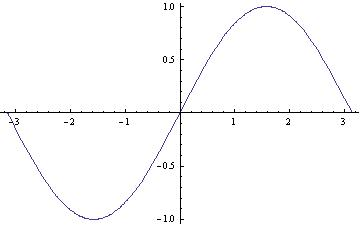
\includegraphics[height=2.5in, width=3.5in]{sin_x.jpg}
\caption{Enjoyment and fun}
\end{figure}

Vestibulum ut urna eu turpis accumsan hendrerit. Mauris in mi sed eros auctor blandit. Nullam sit amet mauris vel eros aliquam pretium. Cras fermentum tortor. Sed egestas vulputate diam. Aenean sem dui, tincidunt a, ullamcorper eget, pharetra ac, tortor. In at sem vel elit bibendum convallis. Aenean ut enim vel leo malesuada dapibus. Etiam odio dolor, sollicitudin a, nonummy nec, tristique et, augue. Morbi ipsum. Aliquam venenatis. Proin orci. Duis sed quam eget turpis interdum feugiat.

\subsection{Hypothesis}  


Glossy prints of good reproducible quality, either black or white or color may be used. Photographs can be printed on 8 1/2$''$ x 11$''$ glossy finish paper, however, margin and page number requirements as stated above still apply for pages containing photographs. When attaching photographs to paper, double-sided tape may be used which causes the least amount of damage to the original paper.

The format of footnotes and the bibliography are to be prepared in accordance with standard practice in the field in which one is working. Documentation formatting style must be discussed with and accepted by the advisor. See further information on Reference Styles below.

The suggested typeface for dissertations is 10 to 12 point Arial. Other suggested fonts are Times New Roman and Helvetica. Script and italic fonts should not be used except as needed in the body of the paper. Consistency should be maintained throughout the paper, using the same font for all text, diagrams, etc. on all pages.

Electronic material, such as CDs and multimedia can accompany the dissertation. Each copy should be accompanied with a labeled CD. When bound, these are placed in an envelope in the back of the dissertation.  Oversized materials (pages greater than 8$''$ x 11$''$) can be included in the paper if necessary. Oversized pages should be folded so that 1$''$ on the left hand binding edge remains, allowing the page to be opened once the paper is bound.

The reference style used for formatting the paper must be confirmed with your department and advisor. Frequently used styles are the APA (American Psychological Association), MLA (Modern Language Association) and AMA (American Medical Association) styles. Style guides and manuals are available for each style. Page headers are not to be used.


\chapter{Current Practice}
Three copies of the dissertation (1 original and 2 copies, either xerographic, photocopied, offset or letter quality printer) are to be supplied to the Library. In addition, an abstract independent of the document is to be supplied to the Library. The announcement for Ph.D. dissertation defense is to be given to The Office of the Registrar at least 1½ weeks prior to the defense. A sample defense announcement can be found in sample pages.

You must hand in your dissertation in person to Doris Oliver. If Doris is not available, Nydia Cruz can also accept dissertations. Dissertations cannot be mailed to the Library and cannot be handed in by another person.

Doris Oliver is available to accept dissertations from 9:30am - 1:00pm and 2:00pm - 4:00 pm, M-F. Appointments are not necessary but are highly recommended.

\subsection*\normalsize\emph{Publication Agreement and Survey Forms}

The UMI Publication Agreement Form and a Survey of Earned Doctorates Form are submitted with the dissertation. The forms are available from Doris Oliver and online. Both forms must be completed and returned to Doris Oliver with the final dissertation. The UMI Publication Agreement Form includes the application form. This should be read, filled out and returned to Doris Oliver. The Survey of Earned Doctorates form is available online in two documents: the Survey of Earned Doctorates brochure and the Survey of Earned Doctorates form online.  UMI also provides a brochure on privacy as it relates to dissertations.

\subsection*\normalsize\emph{Use of Previously Published work in your dissertation}

If you are including previously published material as part of your dissertation, either as an appendix or as part of the body of your paper, you must obtain written permission from the publisher to have the work included as part of your paper.   Even if you are the author of the published material, you still must get permission from the publisher.    

Please view the dissertation specifications on the library website for information about UMI/Proquest's guide to copyright and copyright infringement. 

UMI/Proquest also includes information written by Kenneth Crews, a professor at Indiana University on the issue of copyright.  His work covers how to request permission from publishers, and sample permission letters.

\Large It is the responsibility of the student to ensure that all portions of their dissertation adhere to copyright law.  


\normalsize 

\begin{figure}[htp]
\centering
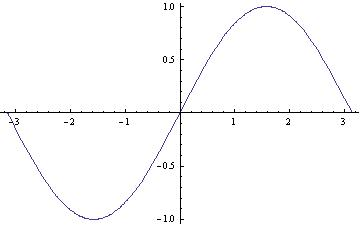
\includegraphics{sin_x.jpg}
\caption{Transverse momentum distributions}\label{fig:erptsqfit}
\end{figure}




\chapter{Case Study}
All information about formatting a dissertation can be found on the library website at www.stevens.edu/library/services/phd.html.  Formatting information gets updated occasionally, so it is always good to check the requirements before submitting your dissertation.  

It is not required, but is strongly suggested that you make an appointment at the library to have the format of your dissertation reviewed before the final submission.  Dissertations can be rejected if they do not adhear to the formatting requirements.   

All information about formatting a dissertation can be found on the library website at www.stevens.edu/library/services/phd.html.  Formatting information gets updated occasionally, so it is always good to check the requirements before submitting your dissertation.  
It is not required, but is strongly suggested that you make an appointment at the library to have the format of your dissertation reviewed before the final submission.  Dissertations can be rejected if they do not adhear to the formatting requirements.   
All information about formatting a dissertation can be found on the library website at www.stevens.edu/library/services/phd.html.  Formatting information gets updated occasionally, so it is always good to check the requirements before submitting your dissertation.  

\begin{table}[htp]

\begin{center}
\begin{tabular}{|l|c|p{3.0in}|}
\hline
\multicolumn{3}{|c|}{Theoretical Dissertation Timeline}\\ \hline
Taskt&Time to Finish&Notes\\ \hline
Problem statement&10 hours&Initially very upbeat.\\ \hline
Research&3 days&Literature search to very previous studies.\\ \hline
Reformulation&4 hours&Presented and accepted by advisor\\ \hline
Research&20 days&Literature search to very previous  studies.\\ \hline
Experiments&14 days&Do some experiments and get results.\\ \hline
Format&1 day&Understand format guidelines for paper.\\ \hline
Write&years&Write the paper.\\ \hline
Revise&not too long&Proof read, etc.\\ \hline
Format&1-3 days&Verify correct report format is used.\\ \hline
See Library&1 hour&Meet with Doris to verify formatting.\\ \hline
Defend&1 day&Defend your research.\\ \hline
Revise&0 hours&It was perfect the first time.\\ \hline
Submit&1 day&Submit final dissertation to the library.\\ \hline
\end{tabular}
\end{center} 

\caption{Table of Tasks}\label{fig:erptsqfit}
\end{table}
It is not required, but is strongly suggested that you make an appointment at the library to have the format of your dissertation reviewed before the final submission.  Dissertations can be rejected if they do not adhear to the formatting requirements.   
All information about formatting a dissertation can be found on the library website at www.stevens.edu/library/services/phd.html.  Formatting information gets updated occasionally, so it is always good to check the requirements before submitting your dissertation.  
It is not required, but is strongly suggested that you make an appointment at the library to have the format of your dissertation reviewed before the final submission.  Dissertations can be rejected if they do not adhear to the formatting requirements.   
All information about formatting a dissertation can be found on the library website at www.stevens.edu/library/services/phd.html.  Formatting information gets updated occasionally, so it is always good to check the requirements before submitting your dissertation.  

It is not required, but is strongly suggested that you make an appointment at the library to have the format of your dissertation reviewed before the final submission.  Dissertations can be rejected if they do not adhear to the formatting requirements.   



\section{Further Analysis}  

\subsection*\normalsize\emph{Paper}
The original copy of the dissertation must be produced on good quality 8 1/2$''$ x 11$''$, 20 pound acid-free white paper. The paper should not be stapled, punched, bound, colored or printed on letterhead.

The two additional copies of the dissertation can be photocopied or produced on copier or laser paper.

\subsection*\normalsize\emph{Ink}
Black ink only is used to print your report.  If a graph or photograph contains color, that is fine. 

Latex is used to help in the printing of formulas.   The following formula would be difficult to reproduce in Microsoft Word: 
 \[
        \frac{d}{dx}\left( \int_{0}^{x} f(u)\,du\right)=f(x).
     \]

This Report was produced by LaTeX\footnote {\LaTeX\ is a fun typesetting program.} written by Barbara Arnett.  Barbara is not an expert with LaTeX, and anyone using LaTeX does not need to use this template.  It is simply provided to help with formatting, specifically with page numbers and images.  


%this subsection heading below will not show up in the table of contents.
\subsection*\normalsize\emph{Graphics} 

Graph paper may be used for original drawings, charts or illustrations. Original drawings may be in color or black and white, however, color is allowed for illustrations only; all text must appear in black. The original thesis must contain the original graphic or illustration, not a photocopy of the drawing, graphic or illustration.

If formulas and diagrams contain subscript and superscript characters, ensure they are large enough to read when printed in the final paper. 

\begin{figure}[htp]
\centering
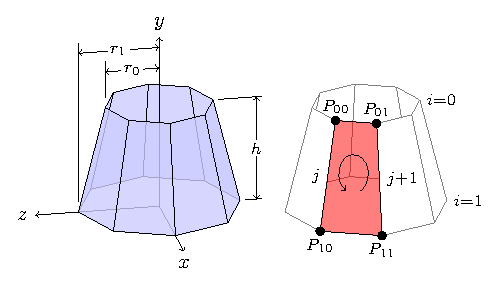
\includegraphics{3d-cone.pdf}
\caption{3D Cone}\label{fig:3d-cone}
\end{figure}

Photographs
Glossy prints of good reproducible quality, either black or white or color may be used. Photographs can be printed on 8 1/2$''$ x 11$''$ glossy finish paper, however, margin and page number requirements as stated above still apply for pages containing photographs. When attaching photographs to paper, double-sided tape may be used which causes the least amount of damage to the original paper. 

Graphics that are oriented in a landscape position must be done in a manner that retains the page numbering in the upper right hand corner, as shown in figure 3.2.  This can be difficult in Microsoft Word, but it is possible.  To do this in Microsoft Word, create a new section, change the page to landscape, and place the page number in a text box.  The text box then is rotated on the landscape page.    Then begin a new section and resume portrait orientation.

\begin{sidewaysfigure}
\centering
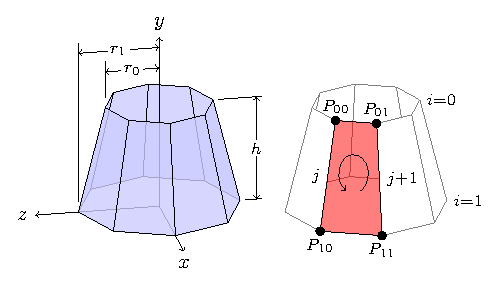
\includegraphics[height=5.0in, width=7.5in]{3d-cone.pdf}
\caption{This is an example of a landscape image within a page.  Note that the page number remains in the upper right hand corner of the page when the page is in the portrait position.}
\end{sidewaysfigure}




\chapter{Recommendations}

Glossy prints of good reproducible quality, either black or white or color may be used. Photographs can be printed on 8$''$ x 11$''$ glossy finish paper, however, margin and page number requirements as stated above still apply for pages containing photographs. When attaching photographs to paper, double-sided tape may be used which causes the least amount of damage to the original paper.

The format of footnotes and the bibliography are to be prepared in accordance with standard practice in the field in which one is working. Documentation formatting style must be discussed with and accepted by the advisor. See further information on Reference Styles below.

The suggested typeface for dissertations is 10 to 12 point Arial. Other suggested fonts are Times New Roman and Helvetica. Script and italic fonts should not be used except as needed in the body of the paper. Consistency should be maintained throughout the paper, using the same font for all text, diagrams, etc. on all pages.

Electronic material, such as CDs and multimedia can accompany the dissertation. Each copy should be accompanied with a labeled CD. When bound, these are placed in an envelope in the back of the dissertation.  Oversized materials (pages greater than 8 1/2$''$ x 11$''$) can be included in the paper if necessary. Oversized pages should be folded so that 1$''$ on the left hand binding edge remains, allowing the page to be opened once the paper is bound.

The reference style used for formatting the paper must be confirmed with your department and advisor. Frequently used styles are the APA (American Psychological Association), MLA (Modern Language Association) and AMA (American Medical Association) styles. Style guides and manuals are available for each style. Page headers are not to be used.


\section{The Focus Group}    

Glossy prints of good reproducible quality, either black or white or color may be used. Photographs can be printed on 8 1/2$''$ x 11$''$ glossy finish paper, however, margin and page number requirements as stated above still apply for pages containing photographs. When attaching photographs to paper, double-sided tape may be used which causes the least amount of damage to the original paper.

The format of footnotes and the bibliography are to be prepared in accordance with standard practice in the field in which one is working. Documentation formatting style must be discussed with and accepted by the advisor. See further information on Reference Styles below.

The suggested typeface for dissertations is 10 to 12 point Arial. Other suggested fonts are Times New Roman and Helvetica. Script and italic fonts should not be used except as needed in the body of the paper. Consistency should be maintained throughout the paper, using the same font for all text, diagrams, etc. on all pages.

\begin{table}[htp]

\begin{center}
\begin{tabular}{|l|c|p{3.0in}|}
\hline
\multicolumn{2}{|c|}{Another Timeline}\\ \hline
Taskt&Notes\\ \hline
Problem statement&Initially very upbeat.\\ \hline
Research&Literature search to very previous studies.\\ \hline
Reformulation&Presented and accepted by advisor\\ \hline
Research&Literature search to very previous  studies.\\ \hline
Experiments&Do some experiments and get results.\\ \hline
Format&Understand format guidelines for paper.\\ \hline
Write&Write the paper.\\ \hline
Revise&Proof read, etc.\\ \hline
Format&Verify correct report format is used.\\ \hline
See Library&Meet with Doris to verify formatting.\\ \hline
Defend&Defend your research.\\ \hline
Revise&It was perfect the first time.\\ \hline
Submit&Submit final dissertation to the library.\\ \hline
\end{tabular}
\end{center} 
\caption{Timeline 2}\label{fig:erptsqfit}
\end{table}

Electronic material, such as CDs and multimedia can accompany the dissertation. Each copy should be accompanied with a labeled CD. When bound, these are placed in an envelope in the back of the dissertation.  Oversized materials (pages greater than 8 1/2$''$ x 11$''$) can be included in the paper if necessary. Oversized pages should be folded so that 1½" on the left hand binding edge remains, allowing the page to be opened once the paper is bound.

The reference style used for formatting the paper must be confirmed with your department and advisor. Frequently used styles are the APA (American Psychological Association), MLA (Modern Language Association) and AMA (American Medical Association) styles. Style guides and manuals are available for each style. Page headers are not to be used.

\chapter{Summary and Conclusion}

Glossy prints of good reproducible quality, either black or white or color may be used. Photographs can be printed on 8 1/2$''$ x 11$''$ glossy finish paper, however, margin and page number requirements as stated above still apply for pages containing photographs. When attaching photographs to paper, double-sided tape may be used which causes the least amount of damage to the original paper.

The format of footnotes and the bibliography are to be prepared in accordance with standard practice in the field in which one is working. Documentation formatting style must be discussed with and accepted by the advisor. See further information on Reference Styles below.

The suggested typeface for dissertations is 10 to 12 point Arial. Other suggested fonts are Times New Roman and Helvetica. Script and italic fonts should not be used except as needed in the body of the paper. Consistency should be maintained throughout the paper, using the same font for all text, diagrams, etc. on all pages.

Electronic material, such as CDs and multimedia can accompany the dissertation. Each copy should be accompanied with a labeled CD. When bound, these are placed in an envelope in the back of the dissertation.  Oversized materials (pages greater than 8 1/2$''$ x 11$''$) can be included in the paper if necessary. Oversized pages should be folded so that 1½" on the left hand binding edge remains, allowing the page to be opened once the paper is bound.

The reference style used for formatting the paper must be confirmed with your department and advisor. Frequently used styles are the APA (American Psychological Association), MLA (Modern Language Association) and AMA (American Medical Association) styles. Style guides and manuals are available for each style. Page headers are not to be used.

\newpage
\addcontentsline{toc}{chapter}{Appendices}	
\addcontentsline{toc}{section}{Appendix A}	
\noindent \textbf{Appendices} \\
%    \chapter{Appendix A}
\noindent \textbf{Appendix A}    %% removed \\
\vspace{12pt}

\noindent Appendices at the end of a dissertation are optional, and depend on the content of the dissertation. There can be one or more appendicies, however they should retain the page numbering requirements for dissertations.  Any concerns about the formatting of an appendix should be brought to Doris Oliver, who can direct you how to format your appendix if you have questions.

\begin{center}
\begin{tabular}{|l|c|p{3.0in}|}
\hline
\multicolumn{3}{|c|}{Theoretical Dissertation Timeline}\\ \hline
Taskt&Time to Finish&Notes\\ \hline
Problem statement&10 hours&Initially very upbeat.\\ \hline
Research&3 days&Literature search to very previous studies.\\ \hline
Reformulation&4 hours&Presented and accepted by advisor\\ \hline
Research&20 days&Literature search to very previous  studies.\\ \hline
Experiments&14 days&Do some experiments and get results.\\ \hline
Format&1 day&Understand format guidelines for paper.\\ \hline
Write&years&Write the paper.\\ \hline
Revise&not too long&Proof read, etc.\\ \hline
Format&1-3 days&Verify correct report format is used.\\ \hline
See Library&1 hour&Meet with Doris to verify formatting.\\ \hline
Defend&1 day&Defend your research.\\ \hline
Revise&0 hours&It was perfect the first time.\\ \hline
Submit&1 day&Submit final dissertation to the library.\\ \hline
\end{tabular}
\end{center} 


% The bibliography is below.  The formatting for the bibliography is not provided here.  Formatting for references can be in 
% the writing style set by the advisor.  Common styles are APA, MLA and Chicago style. 
%
%    if you prefer not to use BibTex, include a line with   \chapter{References} for your bibliography and do not use
%  \bibliography{myrefs} below
%
% 
%
% added this to use bibTex for the bibliography.  If doing bibliography manually, delete

\bibliographystyle{plain}
\newpage
\addcontentsline{toc}{chapter}{Bibliography}		% added May2009
\bibliography{myrefs}


\end{document}
 
